\documentclass[12pt, a4paper]{article} % свойства докуменат
\usepackage[utf8]{inputenc} % хотим нормальную кодировку
\usepackage[T2A]{fontenc} % тип шрифта, по-моему
\usepackage[russian]{babel} % русские буквы и обозначения
\usepackage{graphicx, xcolor} % графика
\usepackage{subfiles} % царская разбивка на много файлов
\usepackage{amsmath} % различные нужные символы, типа \geqslant
\usepackage{amssymb} % еще немного символов
\usepackage{import} % для включения рисунков
\usepackage{titlesec} % для настройки заголовков и секций вообще
\usepackage{caption} % для подписей к рисункам на 2 строки

% комманда для царского добавления в документ векторной графики
\newcommand{\incfig}[1]{%
    \def\svgwidth{\columnwidth}
    \import{figures/}{#1.pdf}
}
\pdfsuppresswarningpagegroup=1

\newcommand\eqdef{\stackrel{\text{\tiny def}}{=}}

% русские знаки нестрогих неравенств
\renewcommand{\le}{\leqslant}
\renewcommand{\ge}{\geqslant}

\newcommand{\sectionbreak}{\clearpage}

\titleformat{\section}{\normalfont\Large\bfseries}{\thesection.}{1em}{}
\titleformat{\subsection}{\normalfont\Large\bfseries}{\thesubsection.}{1em}{}

\DeclareMathOperator{\mymod}{mod}
\DeclareMathOperator*{\res}{res}
\DeclareMathOperator{\normre}{Re}
\DeclareMathOperator{\normim}{Im}
\renewcommand{\Re}{\normre}
\renewcommand{\Im}{\normim}

\graphicspath{figures}

\begin{document}

\subfile{titul.tex}

\tableofcontents

\section{Постановка задачи}
Рассматривается задача Дирихле для уравнения Лапласа
\begin{equation}\label{problem}
	\begin{cases}
		\nabla u\left(x, \, y\right) - \mu u\left(x\, y\right) = 
		f\left(x, \, y\right), \quad \left(x, \, y\right) \in \left[0, \, 1\right] \times \left[0, \, 1\right], \\
		u\left(x, \, 0\right) \equiv u\left(x, \, 1\right) \equiv \xi\left(x\right), \\
		u\left(0, \, y\right) \equiv u\left(1, \, y\right) \equiv \eta\left(y\right), \\ 
		\xi\left(0\right) = \xi\left(1\right) = \eta\left(0\right) = \eta\left(1\right).
	\end{cases}	
\end{equation}

Здесь функция $f\left(\cdot\, , \, \cdot\right)$ непрерывно дифференцируема в $\left[0, \, 1\right]
\times \left[0, \, 1\right]$, функции $\xi\left(\cdot\right), \eta\left(\cdot\right)$ 
непрерывно дифференцируемы на отрезке $\left[0, \, 1\right]$, а вещественный параметр $\mu > 0$.

Для данной задачи нужно построить алгоритм поиска численного решения, основанный
на быстром преобразовании Фурье, а именно необходимо реализовать функцию  
\texttt{solveDirichlet(fHandle, xiHandle, etaHandle, mu, N, M)}
, возвращающую значение решения на сетке размера N на M.
Первые три аргумента функции представляют собой указатели на функции $f\left(\cdot\, , \, \cdot\right), \ \xi\left(\cdot\right), \ \eta\left(\cdot\right)$ соответственно. Затем
передается значение параметра $\mu$ и размер сетки.


\section{Алгоритм решения}

Для этой задачи рассматривается разностная схема, в которой уравнение 
Лапласа принимает вид
\begin{equation} 
\begin{split}
&\dfrac{y_{k+1,l}-2y_{k,l}+y_{k-1,l}}{h_x^2} + 
\dfrac{y_{k,l+1}-2y_{k,l}+y_{k,l-1}}{h_y^2} - \mu y_{k,l} = \phi_{k,l}, \\ \label{approx}
&y_{k,0} = y_{k,M} = \xi_k, \quad y_{0,l} = y_{N,l} = \eta_l, \quad k = 1,\ldots,N-1, \quad l = 1,\ldots,M-1.
\end{split}
\end{equation}

Здесь $h_x = 1/N, \ h_y = 1/M$, значения $y_{k,l}$ аппроксимируют функцию $u(x,y)$ в узлах сетки \\$x_k = \frac{k}{N},\ y_l = \frac{l}{M}, 
y_{k,l} = u\left(x_k, \, y_l\right),\ \phi_{k,l} = f\left(x_k, \, y_l\right),
\xi_k = \xi\left(x_k\right),\ \eta_l = \eta\left(y_l\right).$

Пусть $\left\{a_{s,p}\right\}, \ \left\{b_{s,p}\right\}, \ s = 1,\ldots,N-1, \ p = 1,\ldots,M-1$ задают обратное двумерное преобразование для $y_{k,m}$ и $\phi_{k,m}$ соответствено. Тогда 
$$ y_{k,m}=\sum_{s=0}^{N-1}\sum_{p=0}^{M-1}a_{s,p}e^{-2\pi i \left(\frac{ks}{N} + \frac{mp}{M}\right)}$$
$$ \phi_{k,m}=\sum_{s=0}^{N-1}\sum_{p=0}^{M-1}b_{s,p}e^{-2\pi i \left(\frac{ks}{N} + \frac{mp}{M}\right)}$$

Подставляя эти соотношения в разностную схему (\ref{approx}) и приравнивая коэффициенты при экспонентах, получаем
\begin{equation}
a_{s,p}c_{s,p}= b_{s,p}, \label{ac=b}
\end{equation}
где $$c_{s,p} = -4N^2\sin^2\left(\frac{\pi s}{N}\right)-4M^2\sin^2\left(\frac{\pi p}{M}\right) - \mu.$$

Для выполнения краевых условий нужно специальным образом подобрать значения $\phi_{k,0}, \, \phi_{0,l}$. Для запишем обратное ПФ для
$b_{s,p}$  и представим его в виде сумм
\begin{multline} 
b_{s,p}=\dfrac{1}{MN}\sum_{k=0}^{N-1}\sum_{m=0}^{M-1}\phi_{k,m}e^{2\pi i \left(\frac{ks}{N} + \frac{mp}{M}\right)}= \\
\dfrac{1}{MN}\sum_{l=0}^{M-1}\phi_{0,l}e^{2\pi i \left(\frac{lp}{M}\right)} + 
\dfrac{1}{MN}\sum_{l=0}^{M-1}\phi_{l,0}e^{2\pi i \left(\frac{ls}{N}\right)} - \dfrac{1}{MN}\phi_{0,0} + \overline{b_{s,p}}.\label{b}
\end{multline}
Здесь $\overline{b_{s,p}} = \dfrac{1}{MN}\sum\limits_{k=1}^{N-1}\sum\limits_{m=1}^{M-1}\phi_{k,m}e^{2\pi i \left(\frac{ks}{N} + \frac{mp}{M}\right)}$.
Заметим, что $\overline{b_{s,p}}$ можно вычислить, применив обратное двумерное преобразование преобразование Фурье (функция \texttt{ifft2} в Matlab) к матрице (взяли $\phi_{0,k} = 0, \quad \phi_{l, 0} = 0, \quad k = 0,\ldots,M-1, \quad l = 0,\ldots,N-1$):
\[ 
\begin{pmatrix}
  0 & 0 & \dots & 0 \\
  0 & \phi_{1,1} & \dots & \phi_{1,M-1} \\
  \hdotsfor{4} \\
  0 & \phi_{N-1,1} & \dots & \phi_{N-1, M-1}
\end{pmatrix}
\]

Так как
$$ y_{0,m} = \eta_m =  \sum_{s=0}^{N-1}\sum_{p=0}^{M-1}a_{s,p}e^{-2\pi i \left(\frac{mp}{M}\right)} = 
\sum_{s=0}^{N-1}\sum_{p=0}^{M-1}\dfrac{b_{s,p}}{c_{s,p}}e^{-2\pi i \left(\frac{mp}{M}\right)},$$
$$  y_{k,0} = \xi_k = \sum_{s=0}^{N-1}\sum_{p=0}^{M-1}a_{s,p}e^{-2\pi i \left(\frac{ks}{N}\right)} = 
\sum_{s=0}^{N-1}\sum_{p=0}^{M-1}\dfrac{b_{s,p}}{c_{s,p}}e^{-2\pi i \left(\frac{ks}{N}\right)},$$
подставляя (\ref{b}) в эти выражения, получим систему линейных алгебраических уравнений относительно
$\phi_{0,0}, \ldots, \phi_{0,M-1}, \phi_{1,0}, \ldots, \phi_{N-1,0}$:
\begin{multline}
\eta_m = \dfrac{1}{MN}\sum_{l=0}^{M-1}\phi_{0,l}\sum_{s=0}^{N-1}\sum_{p=0}^{M-1}\dfrac{1}{c_{s,p}}e^{-2\pi i\frac{mp}{M}}e^{2\pi i\frac{lp}{M}} \\
+ \dfrac{1}{MN}\sum_{l=1}^{N-1}\phi_{l,0}\sum_{s=0}^{N-1}\sum_{p=0}^{M-1}\dfrac{1}{c_{s,p}}e^{-2\pi i\frac{mp}{M}}e^{2\pi i\frac{ls}{N}}
- \sum_{s=0}^{N-1}\sum_{p=0}^{M-1}\dfrac{\overline{b_{s,p}}}{c_{s,p}}e^{-2\pi i\frac{mp}{M}}, \quad m = 0,\ldots,M-1
\end{multline}
\begin{multline}
\xi_k = \dfrac{1}{MN}\sum_{l=0}^{M-1}\phi_{0,l}\sum_{s=0}^{N-1}\sum_{p=0}^{M-1}\dfrac{1}{c_{s,p}}e^{-2\pi i\frac{ks}{N}}e^{2\pi i\frac{lp}{M}} \\
+ \dfrac{1}{MN}\sum_{l=1}^{N-1}\phi_{l,0}\sum_{s=0}^{N-1}\sum_{p=0}^{M-1}\dfrac{1}{c_{s,p}}e^{-2\pi i\frac{ks}{N}}e^{2\pi i\frac{ls}{N}}
- \sum_{s=0}^{N-1}\sum_{p=0}^{M-1}\dfrac{\overline{b_{s,p}}}{c_{s,p}}e^{-2\pi i\frac{ks}{N}}, \quad k = 1,\ldots,N-1
\end{multline}

Так как $\xi_0 = \eta_0$ по условию задачи, то уравнение на $\xi_0$ не было включено в систему.
Для вычисления коэффициентов вида 
$\dfrac{1}{MN}\sum\limits_{s=0}^{N-1}\sum\limits_{p=0}^{M-1}\dfrac{1}{c_{s,p}}e^{-2\pi i\frac{mp}{M}}e^{2\pi i\frac{lp}{M}}$ достаточно
просуммировать матрицу $\left\{\frac{1}{c_{s,p}}\right\}$ по $s$, применить обратное преобразование по $p$ с помощью функции \texttt{fft} и циклически сдвинуть на $m$ вправо.

Коэффициенты вида 
$\dfrac{1}{MN}\sum\limits_{s=0}^{N-1}\sum\limits_{p=0}^{M-1}\dfrac{1}{c_{s,p}}e^{-2\pi i\frac{mp}{M}}e^{2\pi i\frac{ls}{N}}$ 
вычисляются последовательным применением прямого преобразования Фурье к строкам матрицы  $\left\{\frac{1}{c_{s,p}}\right\}$, а затем
обратного преобразования (\texttt{ifft}) к её столбцам.

Правая часть системы вычиляется так же с помощью прямого преобразования \texttt{fft}.

Решив систему, построим матрицу $\left\{\phi_{k,m}\right\},\ k = 1,\ldots,N-1, \ m = 1,\ldots,M-1$.
Применяя к ней двумерное обратное преобразование Фурье (\texttt{ifft2}), находим матрицу
 $\left\{b_{s,p}\right\},\ s = 1,\ldots,N-1, \ p = 1,\ldots,M-1$.
С помощью формулы (\ref{ac=b}) вычислим значения $\left\{a_{s,p}\right\},\ s = 1,\ldots,N-1, \ p = 1,\ldots,M-1$ и применим к ним
прямое преобразование Фурье \texttt{fft2}, найдя тем самым искомое решение 
$\left\{y_{k,m}\right\},\ k = 1,\ldots,N-1, \ m = 1,\ldots,M-1$.

\section {Вычисление аналитического решения}

В этом разделе будет вычислено аналитическое решение задачи (\ref{problem}) для функции 
$f\left(x, \, y\right) = xe^{-4x} + \cos(x) + 2y e^{2y}\sin(2y) = f_1(x) + f_2(y).$ Исходя из вида $f$ решение ищется в виде 
$$u(x, \, y) = u_1(x) + u_2(y), \quad u_1(0) = u_1(1) = u_1^0, \quad u_2(0) = u_2(1) = u_2^0,$$
числа $u_1^0$ и $u_2^0$ известны.

При этих условиях задача (\ref{problem}) распадается на две одномерные краевые задачи
\begin{equation}
\left\{
	\begin{aligned}
	& u_1''-\mu u_1 = xe^{-4x} + \cos(x) \label{bvp1} \\
	& u_1(0) = u_1(1) = u_1^0 
	\end{aligned}	
\right.
\end{equation}

\begin{equation}
\left\{
	\begin{aligned}
	& u_2''-\mu u_2 = 2y e^{2y}\sin(2y) \label{bvp2} \\
	& u_2(0) = u_2(1) = u_2^0 
	\end{aligned}	
\right.
\end{equation}

Общее решение однородного уравнения для обеих задач имеет вид
$$u(x) = c_1 e^{\sqrt{\mu}x} + c_2 e^{-\sqrt{\mu}x}.$$

Далее решаем уравнение методом вариации постоянной: представляем решение в виде 
$u(x) = c_1(x) e^{\sqrt{\mu}x} + c_2(x) e^{-\sqrt{\mu}x}.$
Подставляя данный вид функции в задачи~\eqref{bvp1} и~\eqref{bvp2}.
Легко заметить, что решение имеет вид:

\begin{multline*}
    \operatorname{u_{1}}{\left(x \right)} = - \frac{x e^{- 4 x}}{\mu - 16} +\\
\frac{\mu^{3} u^{0}_{1} e^{\sqrt{\mu} + 4} - \mu^{3} u^{0}_{1} e^{4} - 31 \mu^{2} u^{0}_{1} e^{\sqrt{\mu} + 4} + 31 \mu^{2} u^{0}_{1} e^{4} + \mu^{2} e^{\sqrt{\mu}} + \mu^{2} e^{\sqrt{\mu} + 4} \cos{\left(1 \right)}}{{\left(\mu^{3} e^{2 \sqrt{\mu}} - \mu^{3} - 31 \mu^{2} e^{2 \sqrt{\mu}} + 31 \mu^{2} + 224 \mu e^{2 \sqrt{\mu}} - 224 \mu + 256 e^{2 \sqrt{\mu}} - 256\right) e^{4}}} -\\
\frac{\mu^{2} e^{4} + 224 \mu u^{0}_{1} e^{\sqrt{\mu} + 4} - 224 \mu u^{0}_{1} e^{4} - 23 \mu e^{\sqrt{\mu}}}{{\left(\mu^{3} e^{2 \sqrt{\mu}} - \mu^{3} - 31 \mu^{2} e^{2 \sqrt{\mu}} + 31 \mu^{2} + 224 \mu e^{2 \sqrt{\mu}} - 224 \mu + 256 e^{2 \sqrt{\mu}} - 256\right) e^{4}}} -\\
32 \frac{\mu e^{\sqrt{\mu} + 4} \cos{\left(1 \right)} + 40 \mu e^{4} + 256 u^{0}_{1} e^{\sqrt{\mu} + 4}}{{\left(\mu^{3} e^{2 \sqrt{\mu}} - \mu^{3} - 31 \mu^{2} e^{2 \sqrt{\mu}} + 31 \mu^{2} + 224 \mu e^{2 \sqrt{\mu}} - 224 \mu + 256 e^{2 \sqrt{\mu}} - 256\right) e^{4}}} -\\
\frac{256 u^{0}_{1} e^{4} - 24 e^{\sqrt{\mu}} + 256 e^{\sqrt{\mu} + 4} \cos{\left(1 \right)} - 248 e^{4} e^{\sqrt{\mu} x}}{\left(\mu^{3} e^{2 \sqrt{\mu}} - \mu^{3} - 31 \mu^{2} e^{2 \sqrt{\mu}} + 31 \mu^{2} + 224 \mu e^{2 \sqrt{\mu}} - 224 \mu + 256 e^{2 \sqrt{\mu}} - 256\right) e^{4}}\\
    + \frac{\mu^{3} u^{0}_{1} e^{\sqrt{\mu} + 4} - \mu^{3} u^{0}_{1} e^{4} - 31 \mu^{2} u^{0}_{1} e^{\sqrt{\mu} + 4} + 31 \mu^{2} u^{0}_{1} e^{4} + \mu^{2} e^{\sqrt{\mu} + 4} - \mu^{2} e^{4} \cos{\left(1 \right)}}{\mu^{3} e^{2 \sqrt{\mu}} - \mu^{3} - 31 \mu^{2} e^{2 \sqrt{\mu}} + 31 \mu^{2} + 224 \mu e^{2 \sqrt{\mu}} - 224 \mu + 256 e^{2 \sqrt{\mu}} - 256} -\\
\frac{\mu^{2} + 224 \mu u^{0}_{1} e^{\sqrt{\mu} + 4} - 224 \mu u^{0}_{1} e^{4} - 40 \mu e^{\sqrt{\mu} + 4}}{\mu^{3} e^{2 \sqrt{\mu}} - \mu^{3} - 31 \mu^{2} e^{2 \sqrt{\mu}} + 31 \mu^{2} + 224 \mu e^{2 \sqrt{\mu}} - 224 \mu + 256 e^{2 \sqrt{\mu}} - 256} +\\
\frac{23 \mu + 32 \mu e^{4} \cos{\left(1 \right)} + 256 u^{0}_{1} e^{\sqrt{\mu} + 4}}{\mu^{3} e^{2 \sqrt{\mu}} - \mu^{3} - 31 \mu^{2} e^{2 \sqrt{\mu}} + 31 \mu^{2} + 224 \mu e^{2 \sqrt{\mu}} - 224 \mu + 256 e^{2 \sqrt{\mu}} - 256} -\\
\frac{256 u^{0}_{1} e^{4} + 248 e^{\sqrt{\mu} + 4} - 256 e^{4} \cos{\left(1 \right)} + 24 e^{- \sqrt{\mu} x} e^{\sqrt{\mu} - 4}}{\mu^{3} e^{2 \sqrt{\mu}} - \mu^{3} - 31 \mu^{2} e^{2 \sqrt{\mu}} + 31 \mu^{2} + 224 \mu e^{2 \sqrt{\mu}} - 224 \mu + 256 e^{2 \sqrt{\mu}} - 256} -\\
    \frac{\cos{\left(x \right)}}{\mu + 1} + \frac{8 e^{- 4 x}}{\left(\mu - 16\right)^{2}}
.\end{multline*}

\begin{multline*}
    \displaystyle \operatorname{u_{2}}{\left(y \right)} = - \frac{8 \mu^{2} e^{2 y} \sin{\left(2 y \right)}}{\mu^{4} + 128 \mu^{2} + 4096} - \frac{8 \mu^{2} e^{2 y} \cos{\left(2 y \right)}}{\mu^{4} + 128 \mu^{2} + 4096} - \frac{2 \mu y e^{2 y} \sin{\left(2 y \right)}}{\mu^{2} + 64} +\\ 
    \frac{128 \mu e^{2 y} \sin{\left(2 y \right)}}{\mu^{4} + 128 \mu^{2} + 4096} - \frac{128 \mu e^{2 y} \cos{\left(2 y \right)}}{\mu^{4} + 128 \mu^{2} + 4096} - \frac{16 y e^{2 y} \cos{\left(2 y \right)}}{\mu^{2} + 64}\\
+ \frac{\mu^{4} u^{0}_{2} e^{\sqrt{\mu}} - \mu^{4} u^{0}_{2} - 2 \mu^{3} e^{2} \sin{\left(2 \right)} + 128 \mu^{2} u^{0}_{2} e^{\sqrt{\mu}}}{\mu^{4} e^{2 \sqrt{\mu}} - \mu^{4} + 128 \mu^{2} e^{2 \sqrt{\mu}} - 128 \mu^{2} + 4096 e^{2 \sqrt{\mu}} - 4096} -\\
\frac{128 \mu^{2} u^{0}_{2} + 8 \mu^{2} e^{\sqrt{\mu}} - 8 \mu^{2} e^{2} \sin{\left(2 \right)}}{\mu^{4} e^{2 \sqrt{\mu}} - \mu^{4} + 128 \mu^{2} e^{2 \sqrt{\mu}} - 128 \mu^{2} + 4096 e^{2 \sqrt{\mu}} - 4096} -\\
\frac{24 \mu^{2} e^{2} \cos{\left(2 \right)} + 128 \mu e^{\sqrt{\mu}} - 128 \mu e^{2} \cos{\left(2 \right)} + 4096 u^{0}_{2} e^{\sqrt{\mu}} - 4096 u^{0}_{2} - 512 e^{\sqrt{\mu}}}{\mu^{4} e^{2 \sqrt{\mu}} - \mu^{4} + 128 \mu^{2} e^{2 \sqrt{\mu}} - 128 \mu^{2} + 4096 e^{2 \sqrt{\mu}} - 4096} -\\
\frac{512 \sqrt{2} e^{2} \cos{\left(\frac{\pi}{4} + 2 }\right) e^{\sqrt{\mu}} e^{- \sqrt{\mu} y}}{\mu^{4} e^{2 \sqrt{\mu}} - \mu^{4} + 128 \mu^{2} e^{2 \sqrt{\mu}} - 128 \mu^{2} + 4096 e^{2 \sqrt{\mu}} - 4096} +\\
\frac{\mu^{4} u^{0}_{2} e^{\sqrt{\mu}} - \mu^{4} u^{0}_{2} + 2 \mu^{3} e^{\sqrt{\mu} + 2} \sin{\left(2 \right)} + 128 \mu^{2} u^{0}_{2} e^{\sqrt{\mu}}}{{\mu^{4} e^{2 \sqrt{\mu}} - \mu^{4} + 128 \mu^{2} e^{2 \sqrt{\mu}} - 128 \mu^{2} + 4096 e^{2 \sqrt{\mu}} - 4096}} -\\
\frac{128 \mu^{2} u^{0}_{2} + 24 \mu^{2} e^{\sqrt{\mu} + 2} \cos{\left(2 \right)}}{\mu^{4} e^{2 \sqrt{\mu}} - \mu^{4} + 128 \mu^{2} e^{2 \sqrt{\mu}} - 128 \mu^{2} + 4096 e^{2 \sqrt{\mu}} - 4096} +\\
\frac{8 \mu^{2} e^{\sqrt{\mu} + 2} \sin{\left(2 \right)} - 8 \mu^{2} + 128 \mu e^{\sqrt{\mu} + 2} \cos{\left(2 \right)}}{\mu^{4} e^{2 \sqrt{\mu}} - \mu^{4} + 128 \mu^{2} e^{2 \sqrt{\mu}} - 128 \mu^{2} + 4096 e^{2 \sqrt{\mu}} - 4096} -\\
\frac{128 \mu + 4096 u^{0}_{2} e^{\sqrt{\mu}} - 4096 u^{0}_{2} + 512 \sqrt{2} e^{\sqrt{\mu} + 2} \cos{\left(\frac{\pi}{4} + 2 \right)} + 512 e^{\sqrt{\mu} y}}{\mu^{4} e^{2 \sqrt{\mu}} - \mu^{4} + 128 \mu^{2} e^{2 \sqrt{\mu}} - 128 \mu^{2} + 4096 e^{2 \sqrt{\mu}} - 4096} +\\
    \frac{512 e^{2 y} \sin{\left(2 y \right)}}{\mu^{4} + 128 \mu^{2} + 4096} + \frac{512 e^{2 y} \cos{\left(2 y \right)}}{\mu^{4} + 128 \mu^{2} + 4096}
.\end{multline*} 


\newpage

\section{Графики}

\subsection{Для численного решения}

\noindent
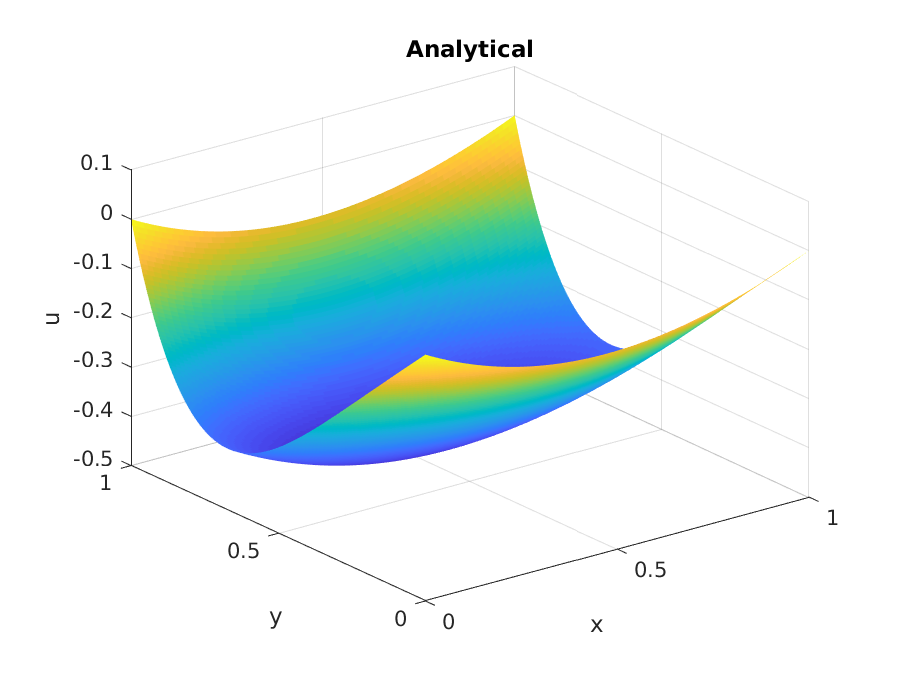
\includegraphics[width=0.51\textwidth]{1_a.eps}
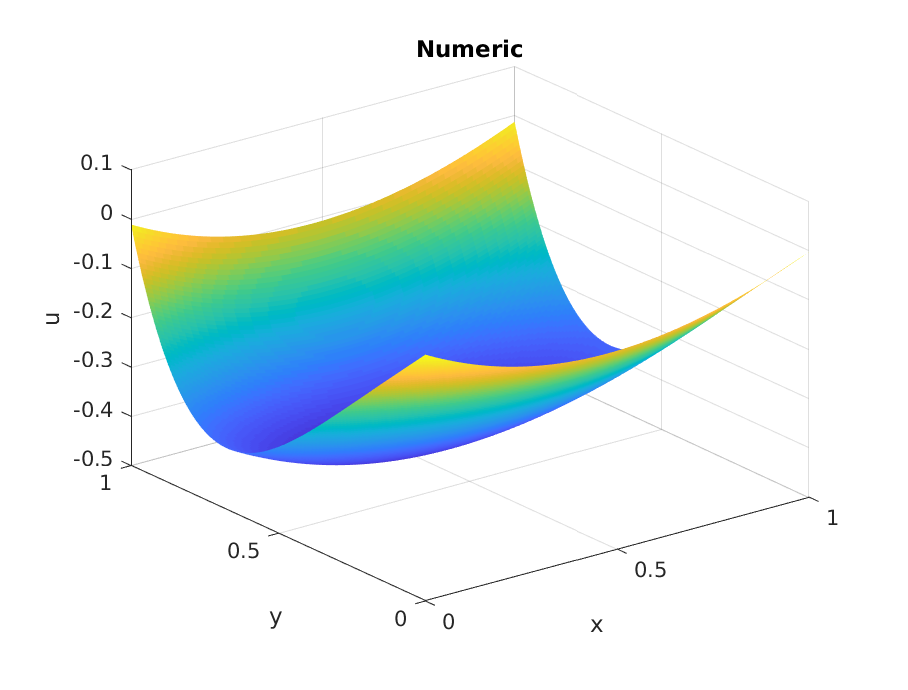
\includegraphics[width=0.51\textwidth]{1_n.eps}
\begin{center}
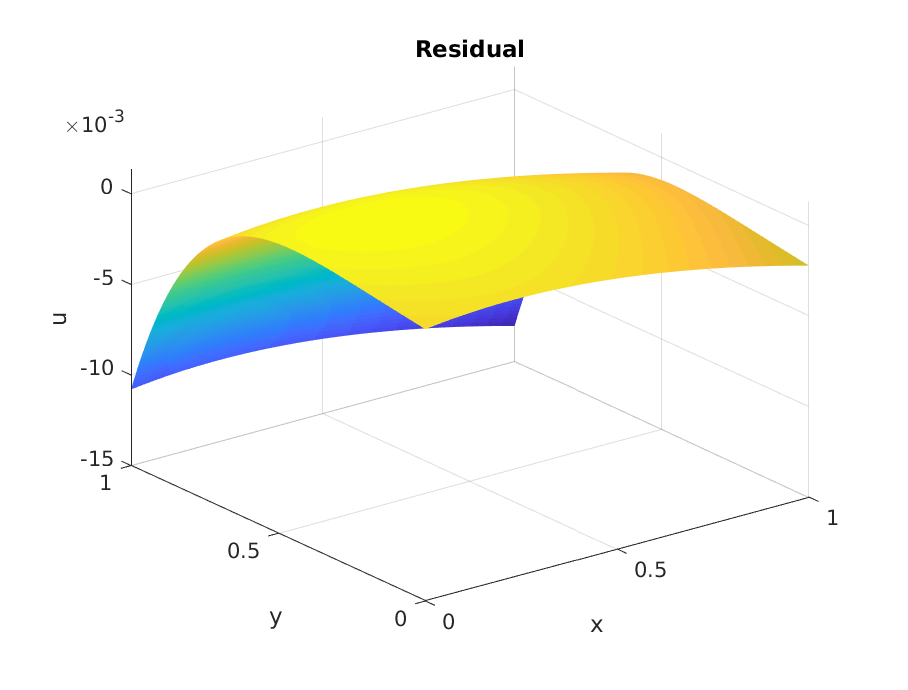
\includegraphics[width=0.7\textwidth]{1_r.eps}

\it{рис. 1 \quad $\mu = 1{,}78, \quad u_1^0 = u_2^0 = 0, \quad M = 156,\ N = 256.$ Максимум невязки~---~$0.013$}
\end{center}

\newpage 

\noindent
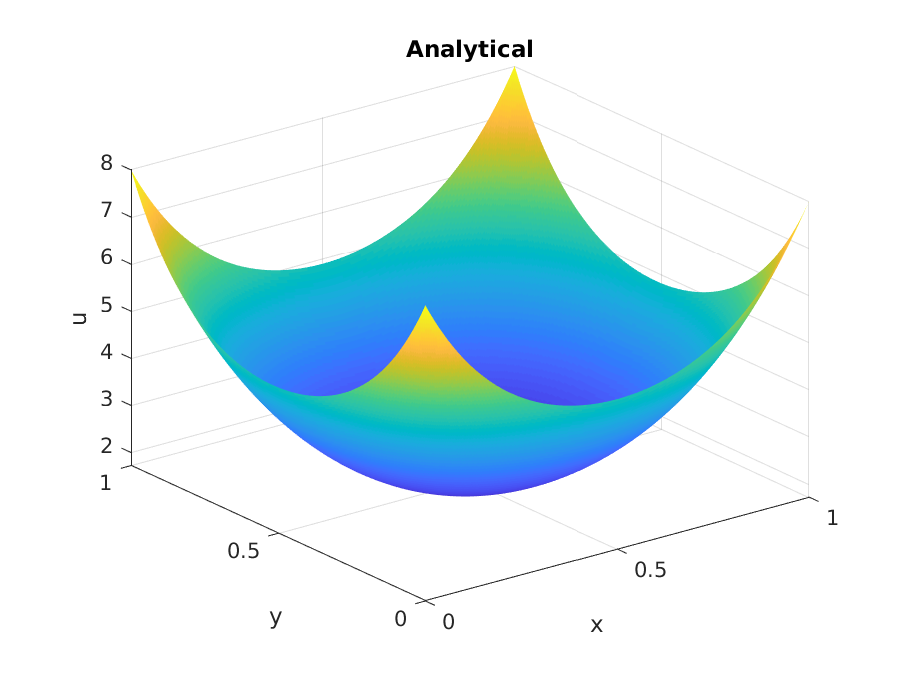
\includegraphics[width=0.51\textwidth]{2_a.eps}
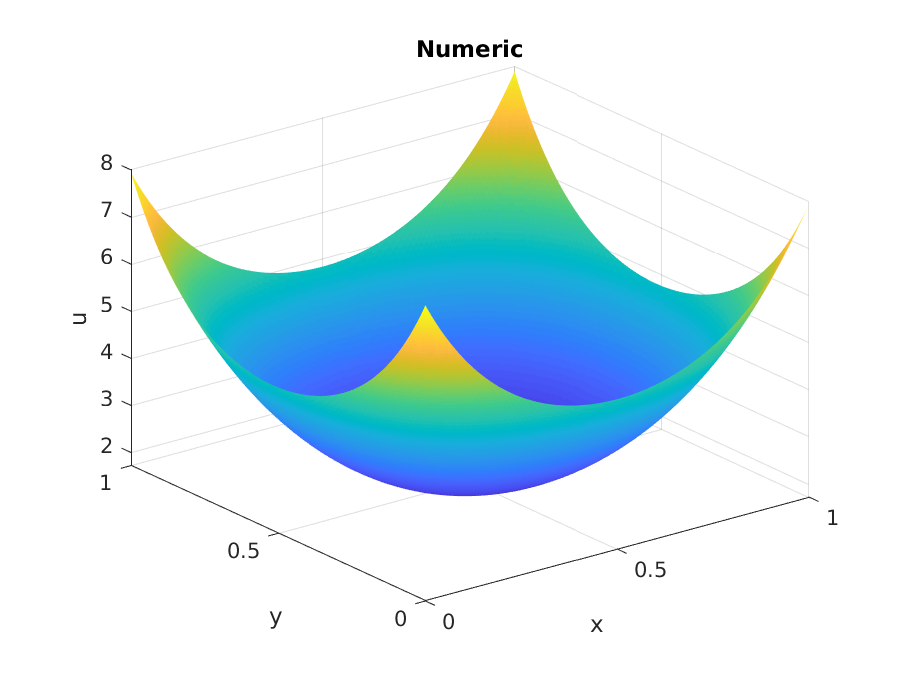
\includegraphics[width=0.51\textwidth]{2_n.eps}
\begin{center}
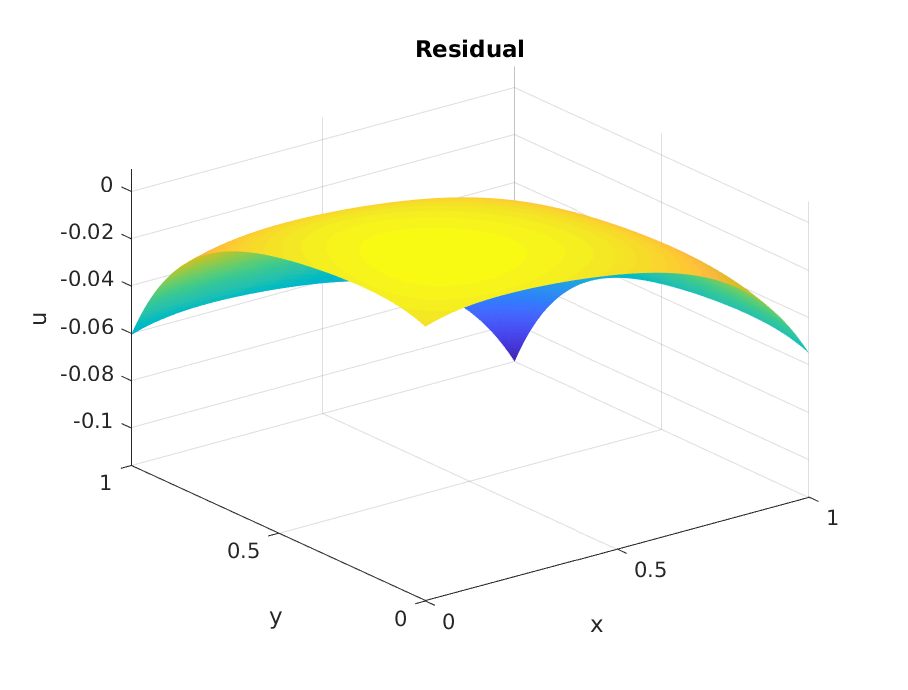
\includegraphics[width=0.7\textwidth]{2_r.eps}

\it{рис. 2 \quad $\mu = 18, \quad u_1^0 = u_2^0 = 4, \quad M = 300,\ N = 300.$ Максимум невязки~---~$0.1169$}
\end{center}

\newpage 

\subsection{Только численное решение}

Пусть $f(x, y) = e^{x^2 + y^4},\ \xi(x) = x(1 - x),\ \eta(y) = y(1-y)$.
В первом случаем шаг сетки $512$, во втором~---~$16$.
\begin{center}
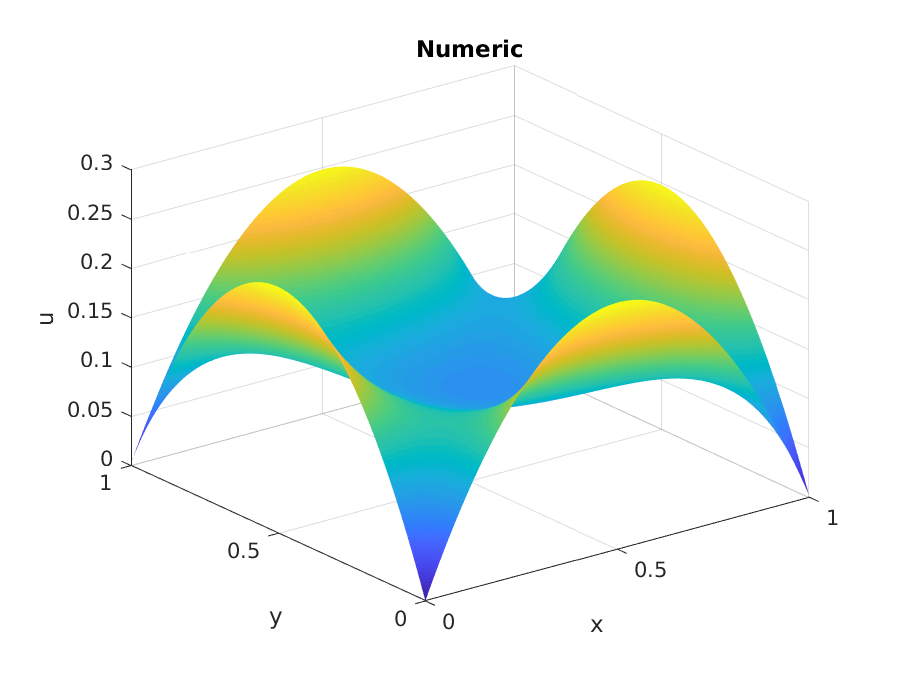
\includegraphics[width=0.81\textwidth]{3_1.eps}\\
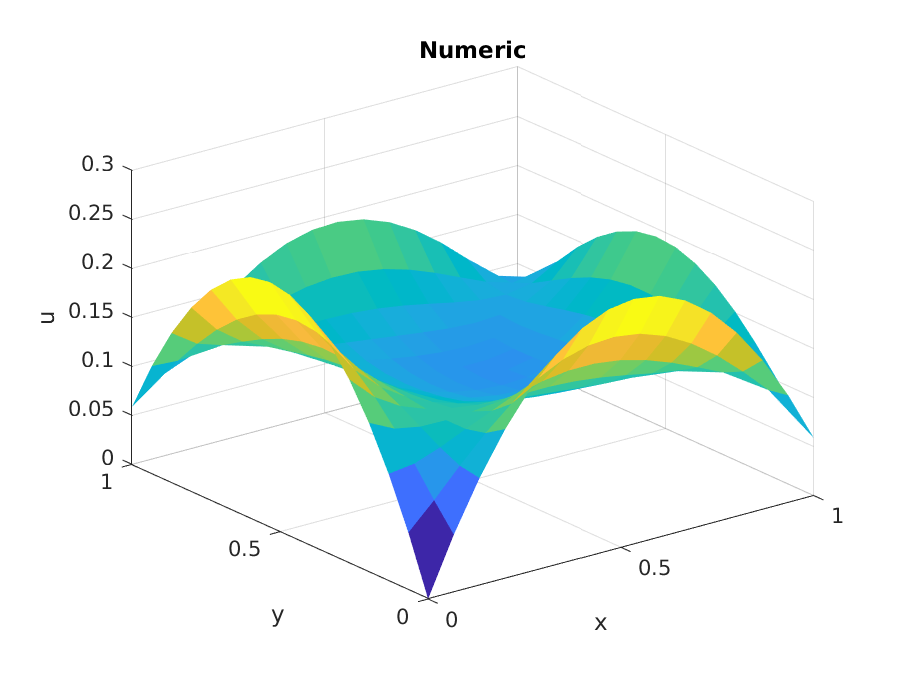
\includegraphics[width=0.81\textwidth]{3_2.eps}
\end{center}

\newpage 

Пусть теперь $f(x, y) = e^{x^2 + 4y^4},\ \xi(x) = x^2(1 - x),\ \eta(y) = y(1-y^3)$.
В первом случаем шаг сетки $512$, во втором~---~$16$.
\begin{center}
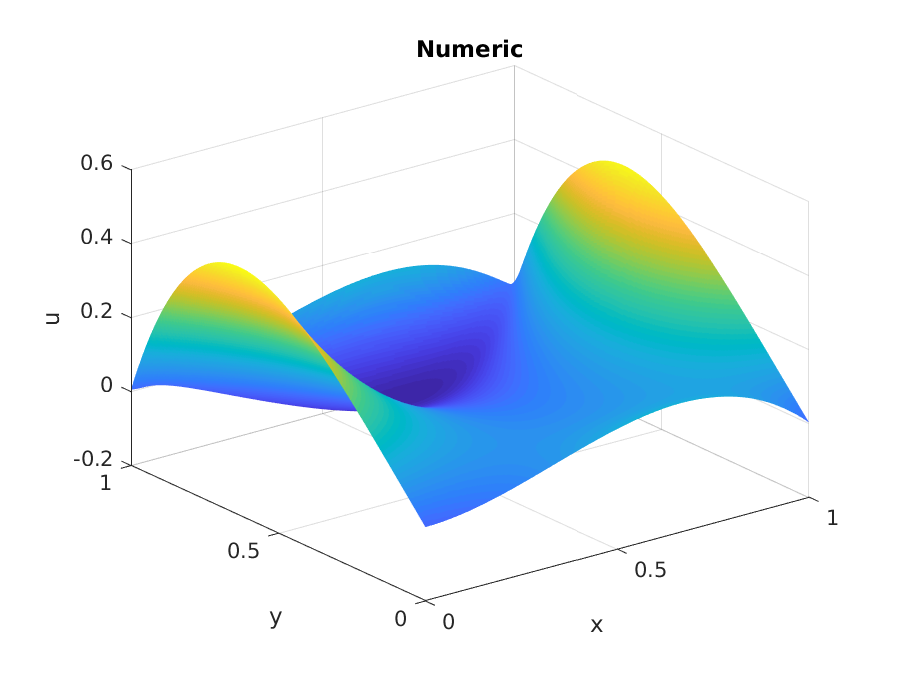
\includegraphics[width=0.81\textwidth]{4_1.eps}\\
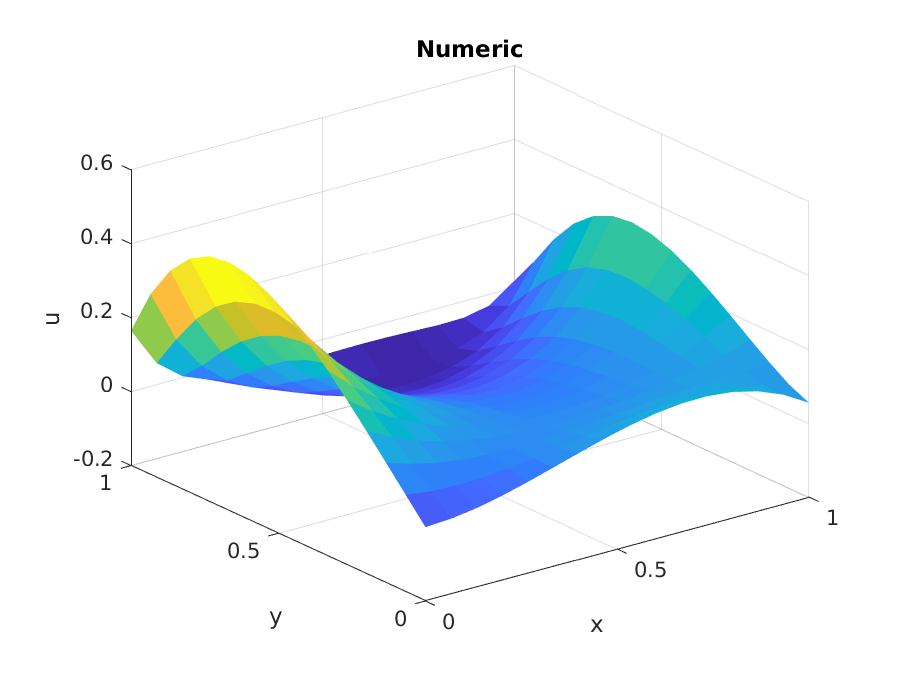
\includegraphics[width=0.81\textwidth]{4_2.eps}
\end{center}


\end{document}
